%%%%%%%%%%%%%%%%%%%%%%%%%%%%%%%%%%%%%%%%%
% baposter Landscape Poster
% LaTeX Template
% Version 1.0 (11/06/13)
%
% baposter Class Created by:
% Brian Amberg (baposter@brian-amberg.de)
%
% This template has been downloaded from:
% http://www.LaTeXTemplates.com
%
% License:
% CC BY-NC-SA 3.0 (http://creativecommons.org/licenses/by-nc-sa/3.0/)
%
%%%%%%%%%%%%%%%%%%%%%%%%%%%%%%%%%%%%%%%%%

%----------------------------------------------------------------------------------------
%	PACKAGES AND OTHER DOCUMENT CONFIGURATIONS
%----------------------------------------------------------------------------------------

\documentclass[portrait,a0paper,fontscale=0.36]{baposter} % Adjust the font scale/size here

\usepackage{graphicx} % Required for including images
\graphicspath{{figures/}} % Directory in which figures are stored

\usepackage{tikz}
\usepackage{amsmath} % For typesetting math
\usepackage{amssymb} % Adds new symbols to be used in math mode
\usepackage[T1]{fontenc}
\usepackage[utf8]{inputenc}
\usepackage{float}
\usepackage[portuguese]{babel}
\usepackage{booktabs} % Top and bottom rules for tables
\usepackage{enumitem} % Used to reduce itemize/enumerate spacing
\usepackage{palatino} % Use the Palatino font
\usepackage[font=small,labelfont=bf]{caption} % Required for specifying captions to tables and figures

\usepackage{multicol} % Required for multiple columns
\setlength{\columnsep}{1.5em} % Slightly increase the space between columns
\setlength{\columnseprule}{0mm} % No horizontal rule between columns

\usepackage{tikz} % Required for flow chart
\usetikzlibrary{shapes,arrows} % Tikz libraries required for the flow chart in the template

\newcommand{\compresslist}{ % Define a command to reduce spacing within itemize/enumerate environments, this is used right after \begin{itemize} or \begin{enumerate}
\setlength{\itemsep}{1pt}
\setlength{\parskip}{0pt}
\setlength{\parsep}{0pt}
}

\definecolor{lightblue}{rgb}{0.145,0.6666,1} % Defines the color used for content box headers

\begin{document}

\begin{poster}
{
headerborder=closed, % Adds a border around the header of content boxes
colspacing=1em, % Column spacing
bgColorOne=white, % Background color for the gradient on the left side of the poster
bgColorTwo=white, % Background color for the gradient on the right side of the poster
borderColor=lightblue, % Border color
headerColorOne=black, % Background color for the header in the content boxes (left side)
headerColorTwo=lightblue, % Background color for the header in the content boxes (right side)
headerFontColor=white, % Text color for the header text in the content boxes
boxColorOne=white, % Background color of the content boxes
textborder=roundedleft, % Format of the border around content boxes, can be: none, bars, coils, triangles, rectangle, rounded, roundedsmall, roundedright, roundedleft or faded
eyecatcher=true, % Set to false for ignoring the left logo in the title and move the title left
headerheight=0.1\textheight, % Height of the header
headershape=rounded, % Specify the rounded corner in the content box headers, can be: rectangle, small-rounded, roundedright, roundedleft or rounded
headerfont=\Large\bf\textsc, % Large, bold and sans serif font in the headers of content boxes
%textfont={\setlength{\parindent}{1.5em}}, % Uncomment for paragraph indentation
linewidth=2pt % Width of the border lines around content boxes
}
%---------------------  -------------------------------------------------------------------
%	TITLE SECTION 
%----------------------------------------------------------------------------------------
%
{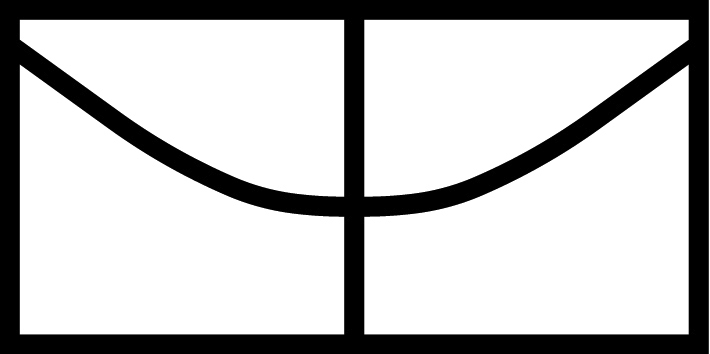
\includegraphics[height=3.3em]{unbblack.jpg}} % First university/lab logo on the left
{\bf{Introdução à Simulação Numérica de Escoamentos de Fluidos Magnéticos}\vspace{0.5em}} % Poster title
{{\{ Ataias Reis - ataiasreis@gmail.com\} \{ Yuri Dumaresq - Y.D.Sobral@mat.unb.br\} \{ Francisco Ricardo - frcunha@unb.br\} \hspace{12pt} Universidade de Brasília, Departamento de Matemática}} % Author names and institution
%{
\includegraphics[height=4em]{logo.png}} % Second university/lab logo on the right


%----------------------------------------------------------------------------------------
%	REFERENCES
%----------------------------------------------------------------------------------------

\headerbox{Referências}{name=references,column=2,above=bottom}{

\renewcommand{\section}[2]{\vskip 0.05em} % Get rid of the default "References" section title
\nocite{*} % Insert publications even if they are not cited in the poster
\small{ % Reduce the font size in this block
%\bibliographystyle{unsrt}
\bibliographystyle{plain}
\bibliography{sample} % Use sample.bib as the bibliography file

}}

%----------------------------------------------------------------------------------------
%	ACKNOLEDGEMENTS
%----------------------------------------------------------------------------------------

\headerbox{Agradecimentos}{name=acknowledgment,column=0,above=bottom}{ % This block is as tall as the reacknoledgmentferences block
Os autores são gratos pelo apoio financeiro a este trabalhado que foi dado pelo CNPq, FAP-DF e Finatec.}

%----------------------------------------------------------------------------------------
%	INTRODUCTION
%----------------------------------------------------------------------------------------

\headerbox{1. Introdução}{name=introduction,column=0,row=0}{

\textbf{Objetivo}\\ - Desenvolver um código de computador que resolva a equação de Navier Stokes \begin{align}
	\left( \frac{\partial {\textbf{v}}}{\partial t}+\textbf{v}\cdot\nabla \textbf{v} \right)=-\nabla p+\frac{1}{\mathit{Re}}\nabla^2 \textbf{v} + \textbf{f}\label{navierstokes},\\
\nabla\cdot\textbf{v}=0\label{navierincompressibilidade}
\end{align} numa cavidade para simular o escoamento de um fluido magnético\cite{RosensweigMagneticFluids} sob ação de um campo magnético aplicado no regime superparamagnético, isto é, \begin{align}
	\mathbf{M} &= \chi \mathbf{H}.
\end{align}

\textbf{Por quê?}\\
 - O caso superparamagnético já é conhecido e serve como validação do código.\\
 - Deseja-se simular a equação de Shliomis\cite{masao1989} \begin{align}
 	\frac{\partial \mathbf{M}}{\partial t} &= -c_1[\mathbf{M} - \mathbf{M}_0]+c_2[(\mathbf{M}\times \mathbf{H})\times\mathbf{M}]\nonumber\\
 	 & + \frac{1}{2}(\nabla\times \mathbf{v})\times \mathbf{M}\label{dMdtadimensional},
 \end{align} uma equação constitutiva para a evolução do campo magnético, e comparar seus resultados com os do caso superparamagnético. \\
\vspace{0.3em} % When there are two boxes, some whitespace may need to be added if the one on the right has more content
}

%----------------------------------------------------------------------------------------
%	METHODS
%----------------------------------------------------------------------------------------

\headerbox{2. Metodologia}{name=method,column=0,below=introduction,above=acknowledgment}{ % This block's bottom aligns with the bottom of the other2 block
As seguintes ferramentas e técnicas foram muito utilizadas no projeto.
\begin{itemize}\compresslist
\item Julia \cite{JuliaProgramming} - uma linguagem de programação
\item GitHub Ferrofluidos\cite{gitHubFerrofluidos} - repositório online do projeto\item Matplotlib \cite{matplotlib} - biblioteca gráfica
\item Time-splitting \cite{chorin68} - técnica para se resolver a equação de Navier Stokes
\item Staggered-grid \cite{hinchLectureNotes} - tipo de malha que é utilizada para diminuir erros no cálculo da pressão
\item Diferenças finitas - método usado para discretizar equações
\end{itemize}

	\begin{center}
		\tikzstyle{help lines}+=[dashed]
\begin{tikzpicture}
%axes
\draw[->] (0,5) -- (xyz cs:y=6);
\draw (0,6.3) node {$y(j)$};
\draw[->] (5,0) -- (xyz cs:x=6);
\draw (6.5,0) node {$x(i)$};
\draw (-0.18,-0.18) node {$O$};
%grid
\draw[style=help lines] (-1,-1) grid +(7,7);
\draw (0,0) grid +(5,5);
%internal p points
\foreach \x in {0.5,1.5,2.5,3.5,4.5}
  \foreach \y in {0.5,1.5,2.5,3.5,4.5}
  {
  \fill (canvas cs:x=\x cm,y=\y cm) circle (2pt);
}
%External p points
\foreach \x in {0.5,1.5,2.5,3.5,4.5}
  \draw (\x,-0.5) circle (2pt);
\foreach \y in {0.5,1.5,2.5,3.5,4.5}
  \draw (5.5,\y) circle (2pt);
\foreach \y in {0.5,1.5,2.5,3.5,4.5}
  \draw (-0.5,\y) circle (2pt);
\foreach \x in {0.5,1.5,2.5,3.5,4.5}
  \draw (\x,5.5) circle (2pt);
%Internal Horizontal Velocities Points
\foreach \x in {-1.2,-0.2,0.8,1.8,2.8,3.8,4.8}
  \foreach \y in {0.5,1.5,2.5,3.5,4.5}
  {
  \draw[->] (\x,\y) -- (\x+0.4,\y);
}
%External Horizontal Velocities Points
\foreach \x in {-.2,0.8,1.8,2.8,3.8}
  \draw[->] (\x,5.5) -- (\x+0.4,5.5);
\foreach \x in {-.2,0.8,1.8,2.8,3.8}
  \draw[->] (\x,-.5) -- (\x+0.4,-.5);
%Internal Vertical Velocities Points
\foreach \x in {0.5,1.5,2.5,3.5,4.5}
  \foreach \y in {-1.2,-0.2,0.8,1.8,2.8,3.8,4.8}
  {
  \draw[->] (\x,\y) -- (\x,\y+0.4);
}
%External Vertical Velocities Points
\foreach \y in {-0.2,0.8,1.8,2.8,3.8}
  \draw[->] (5.5,\y) -- (5.5,\y+0.4);
\foreach \y in {-0.2,0.8,1.8,2.8,3.8}
  \draw[->] (-.5,\y) -- (-.5,\y+0.4);
\end{tikzpicture}
\captionof{figure}{Malha escalonada\label{staggered-grid}}
	\end{center}

}

%%----------------------------------------------------------------------------------------
%%	Integration
%%----------------------------------------------------------------------------------------
%
%\headerbox{4. Integration}{name=anotherresult,column=2,row=0}{
%\begin{center}
%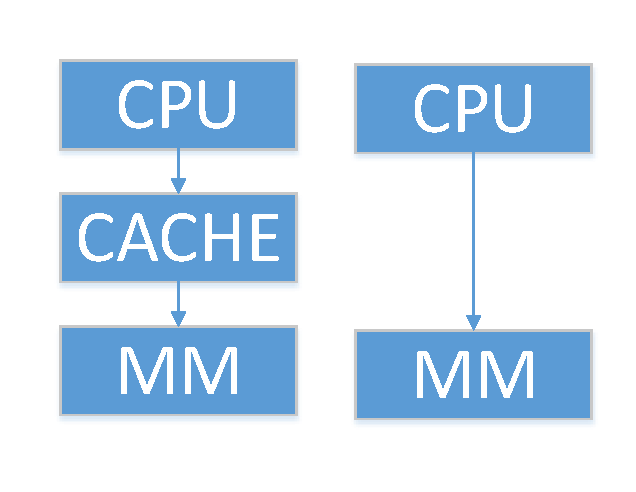
\includegraphics[width=0.9\linewidth]{CacheAndNoCache.pdf}
%\captionof{figure}{Detail of where cache is connected}
%\end{center}
%
%Cache is placed between the CPU and Main Memory. Worst-case time is increased, but it is faster on average.
%
%}

%----------------------------------------------------------------------------------------
%	RESULTS
%----------------------------------------------------------------------------------------

\headerbox{3. Resultados}{name=results,column=1,span=2,row=0}{

\begin{multicols}{2}
%\vspace{1em}

\begin{center}
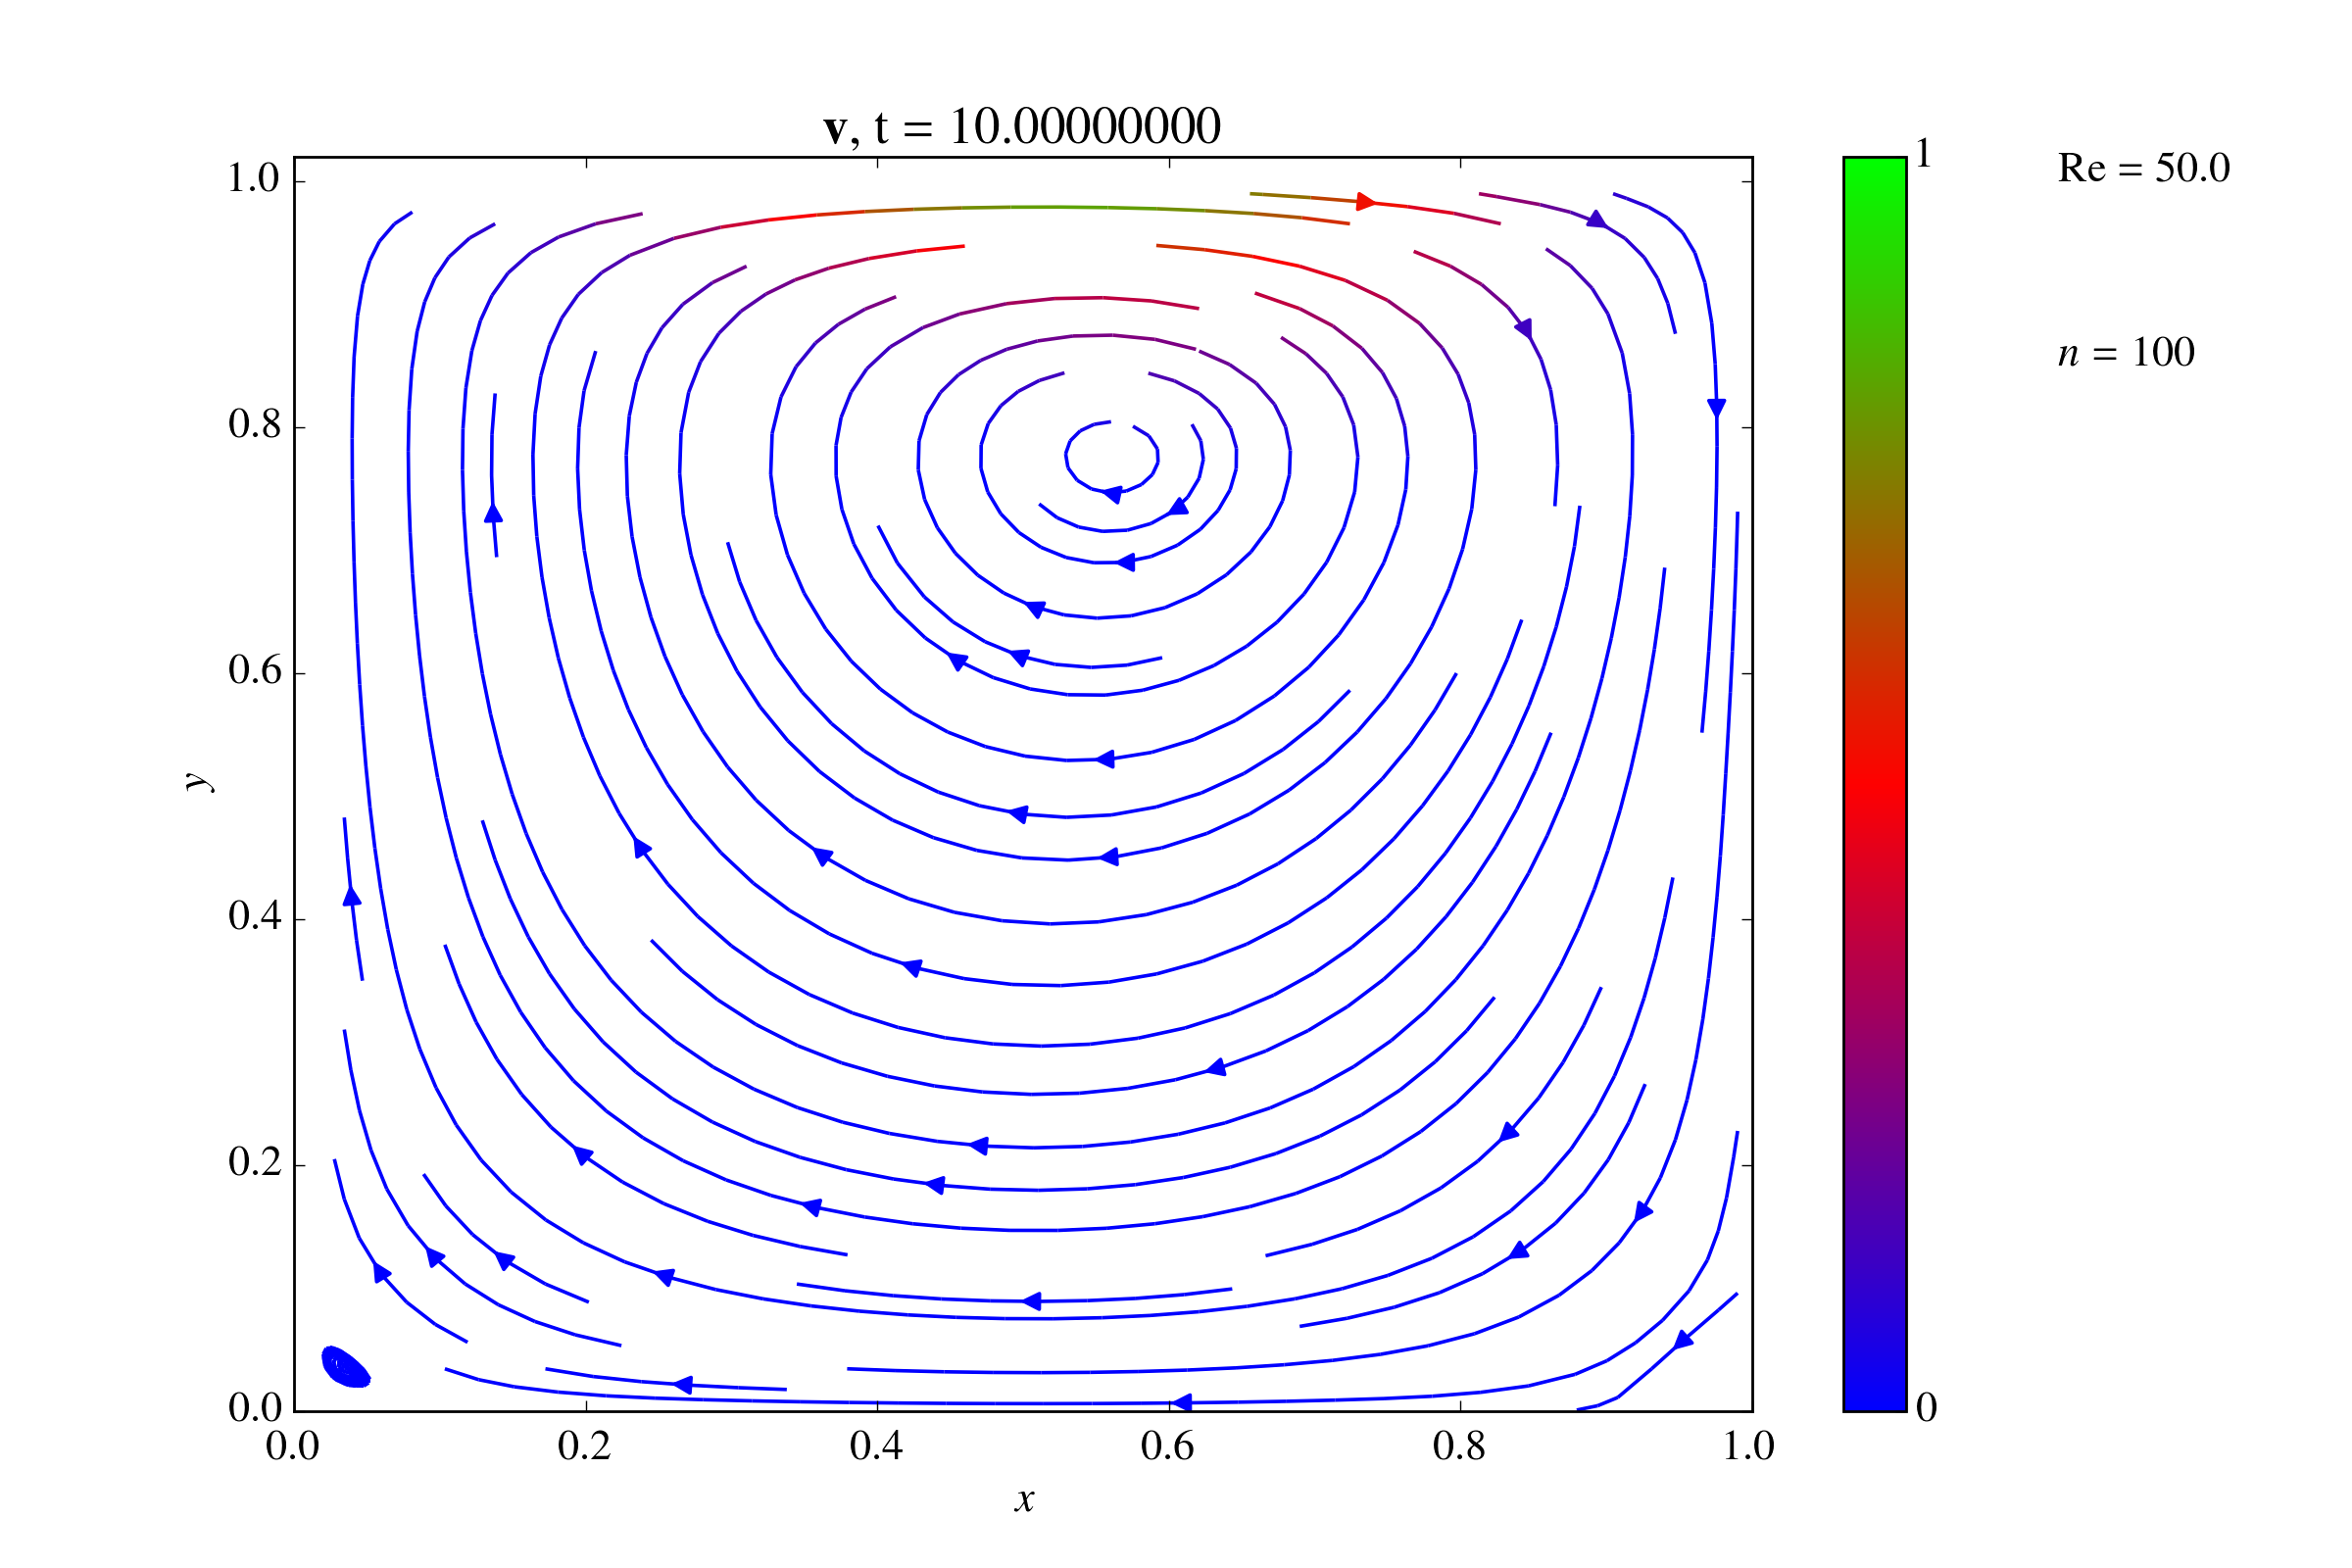
\includegraphics[width=0.8\linewidth]{simulations/vRe50N100Chi01Cpm0T10fps20.png}
\captionof{figure}{Linhas de velocidade em regime sem campo aplicado}
\end{center}

\begin{center}
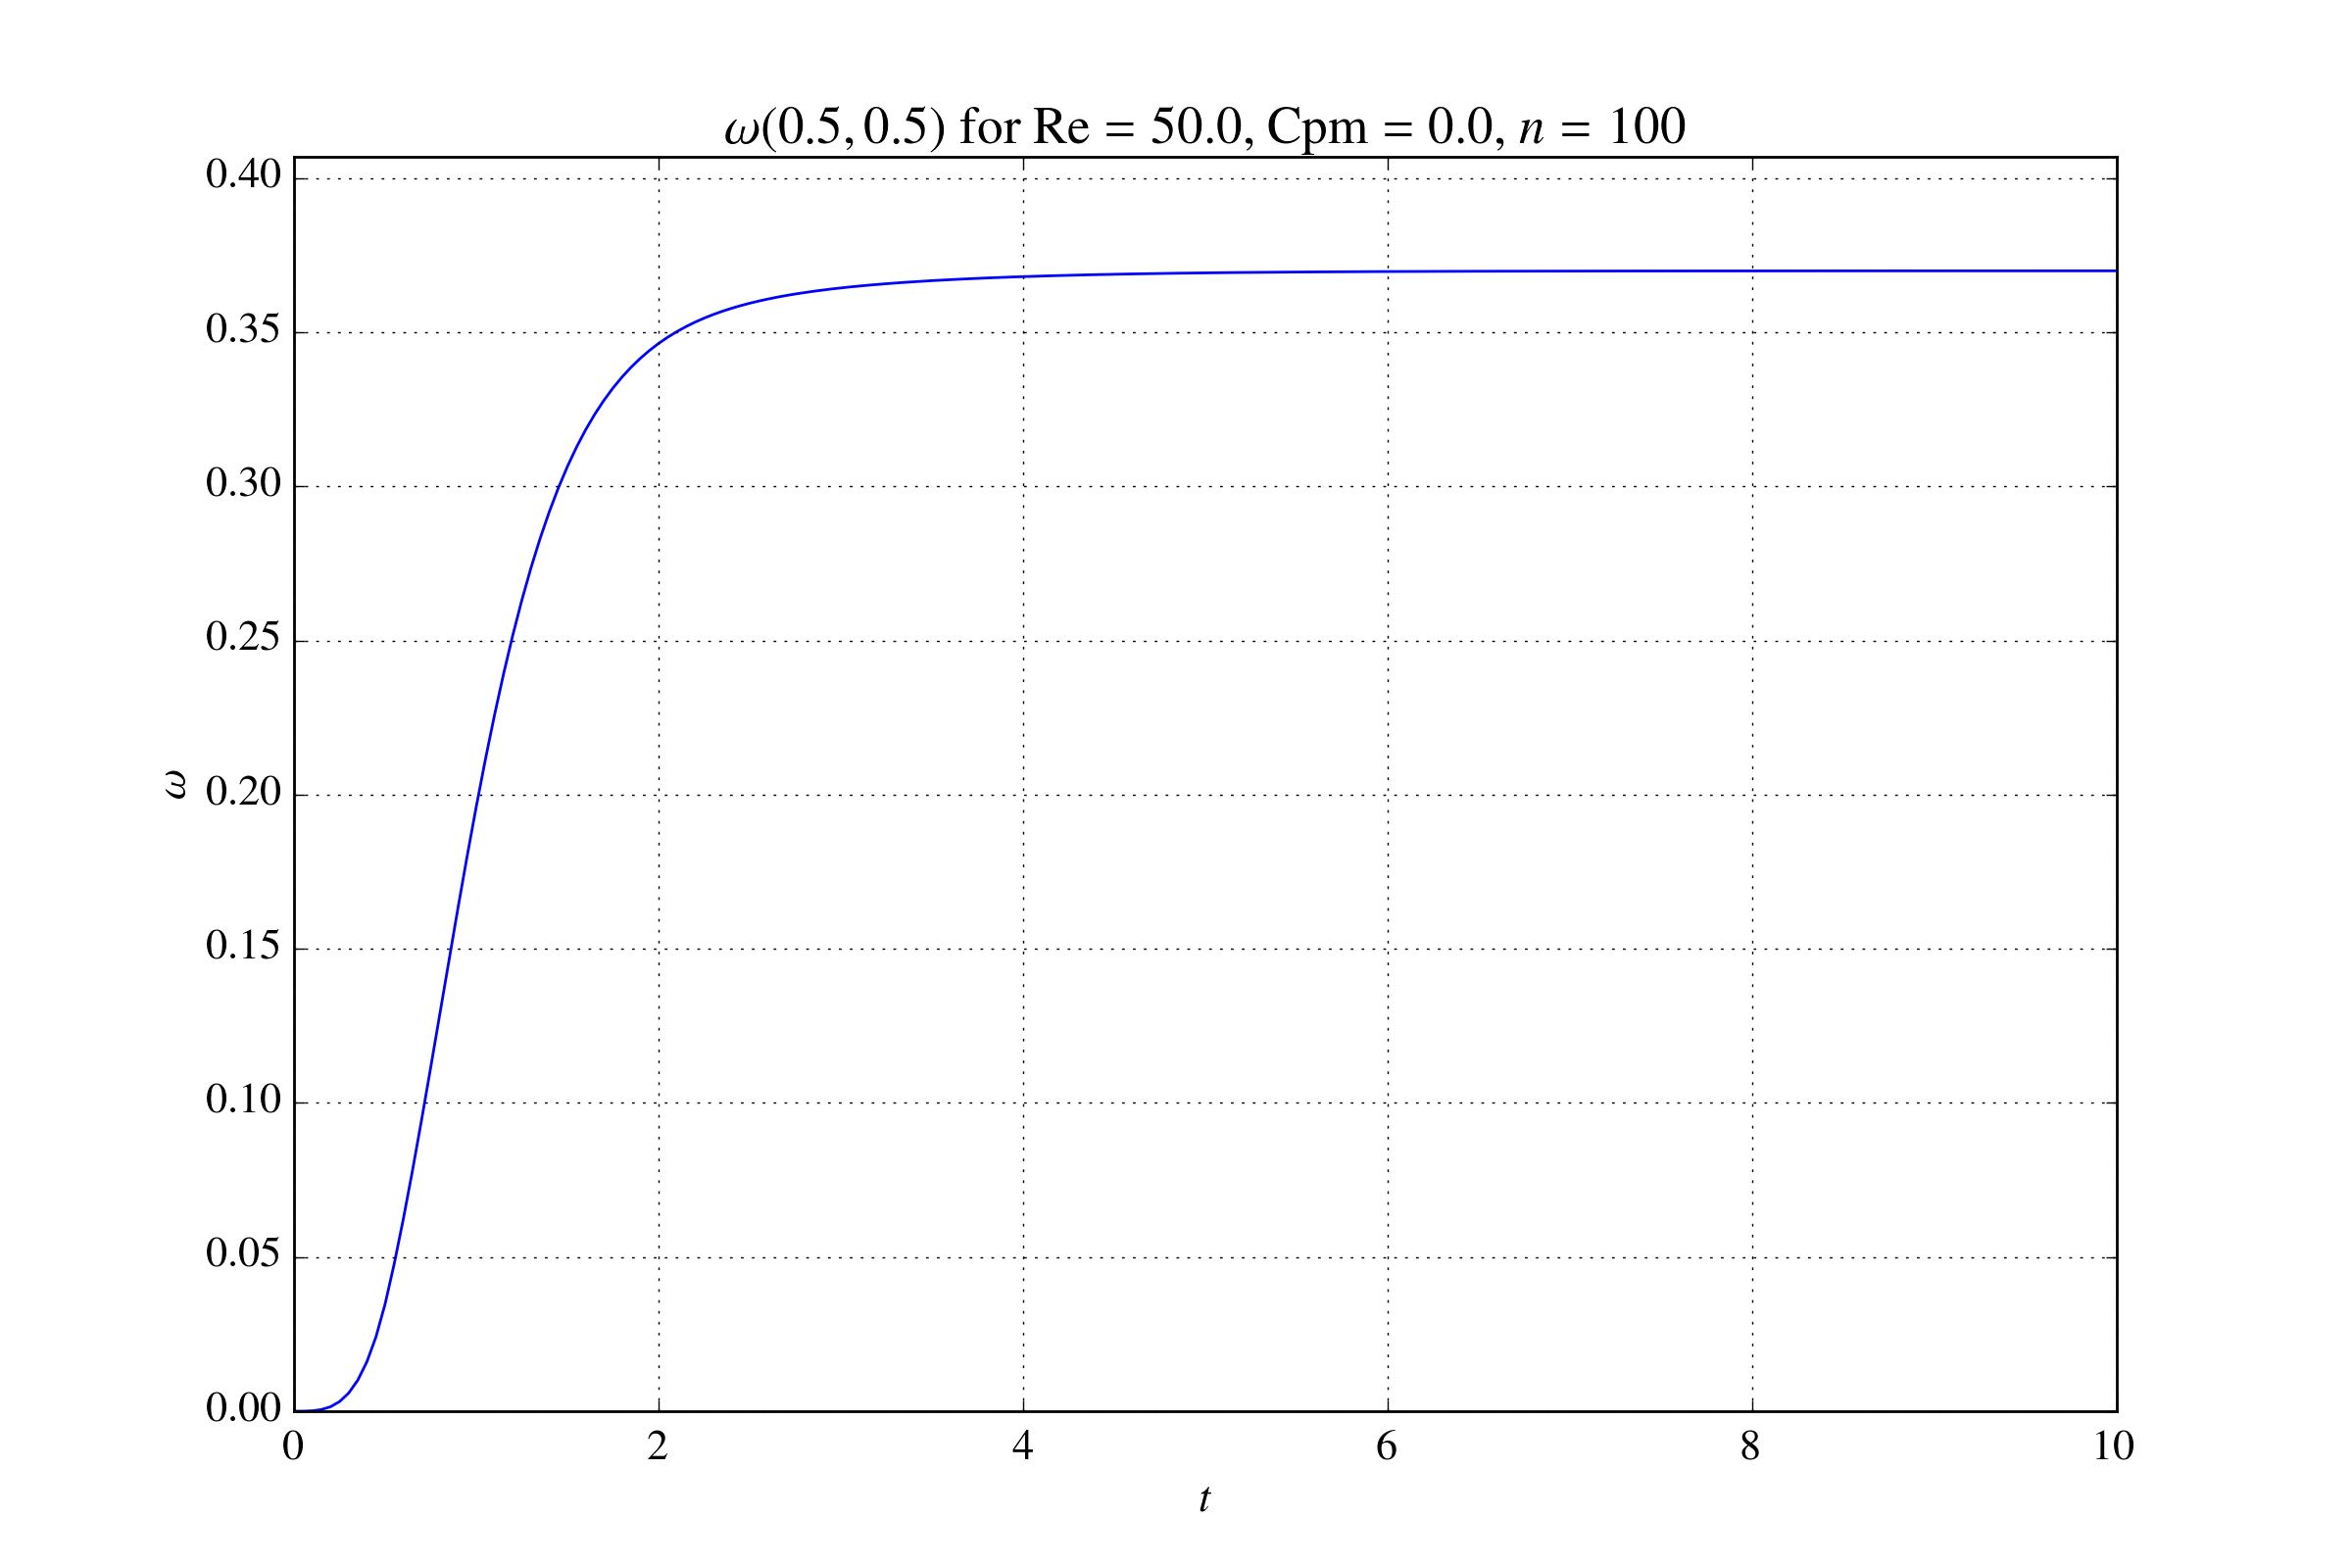
\includegraphics[width=0.8\linewidth]{simulations/vortRe50N100Chi01Cpm0T10fps20.png}
\captionof{figure}{Evolução da vorticidade em (0.5,0.5) sem campo aplicado}
\end{center}

\begin{center}
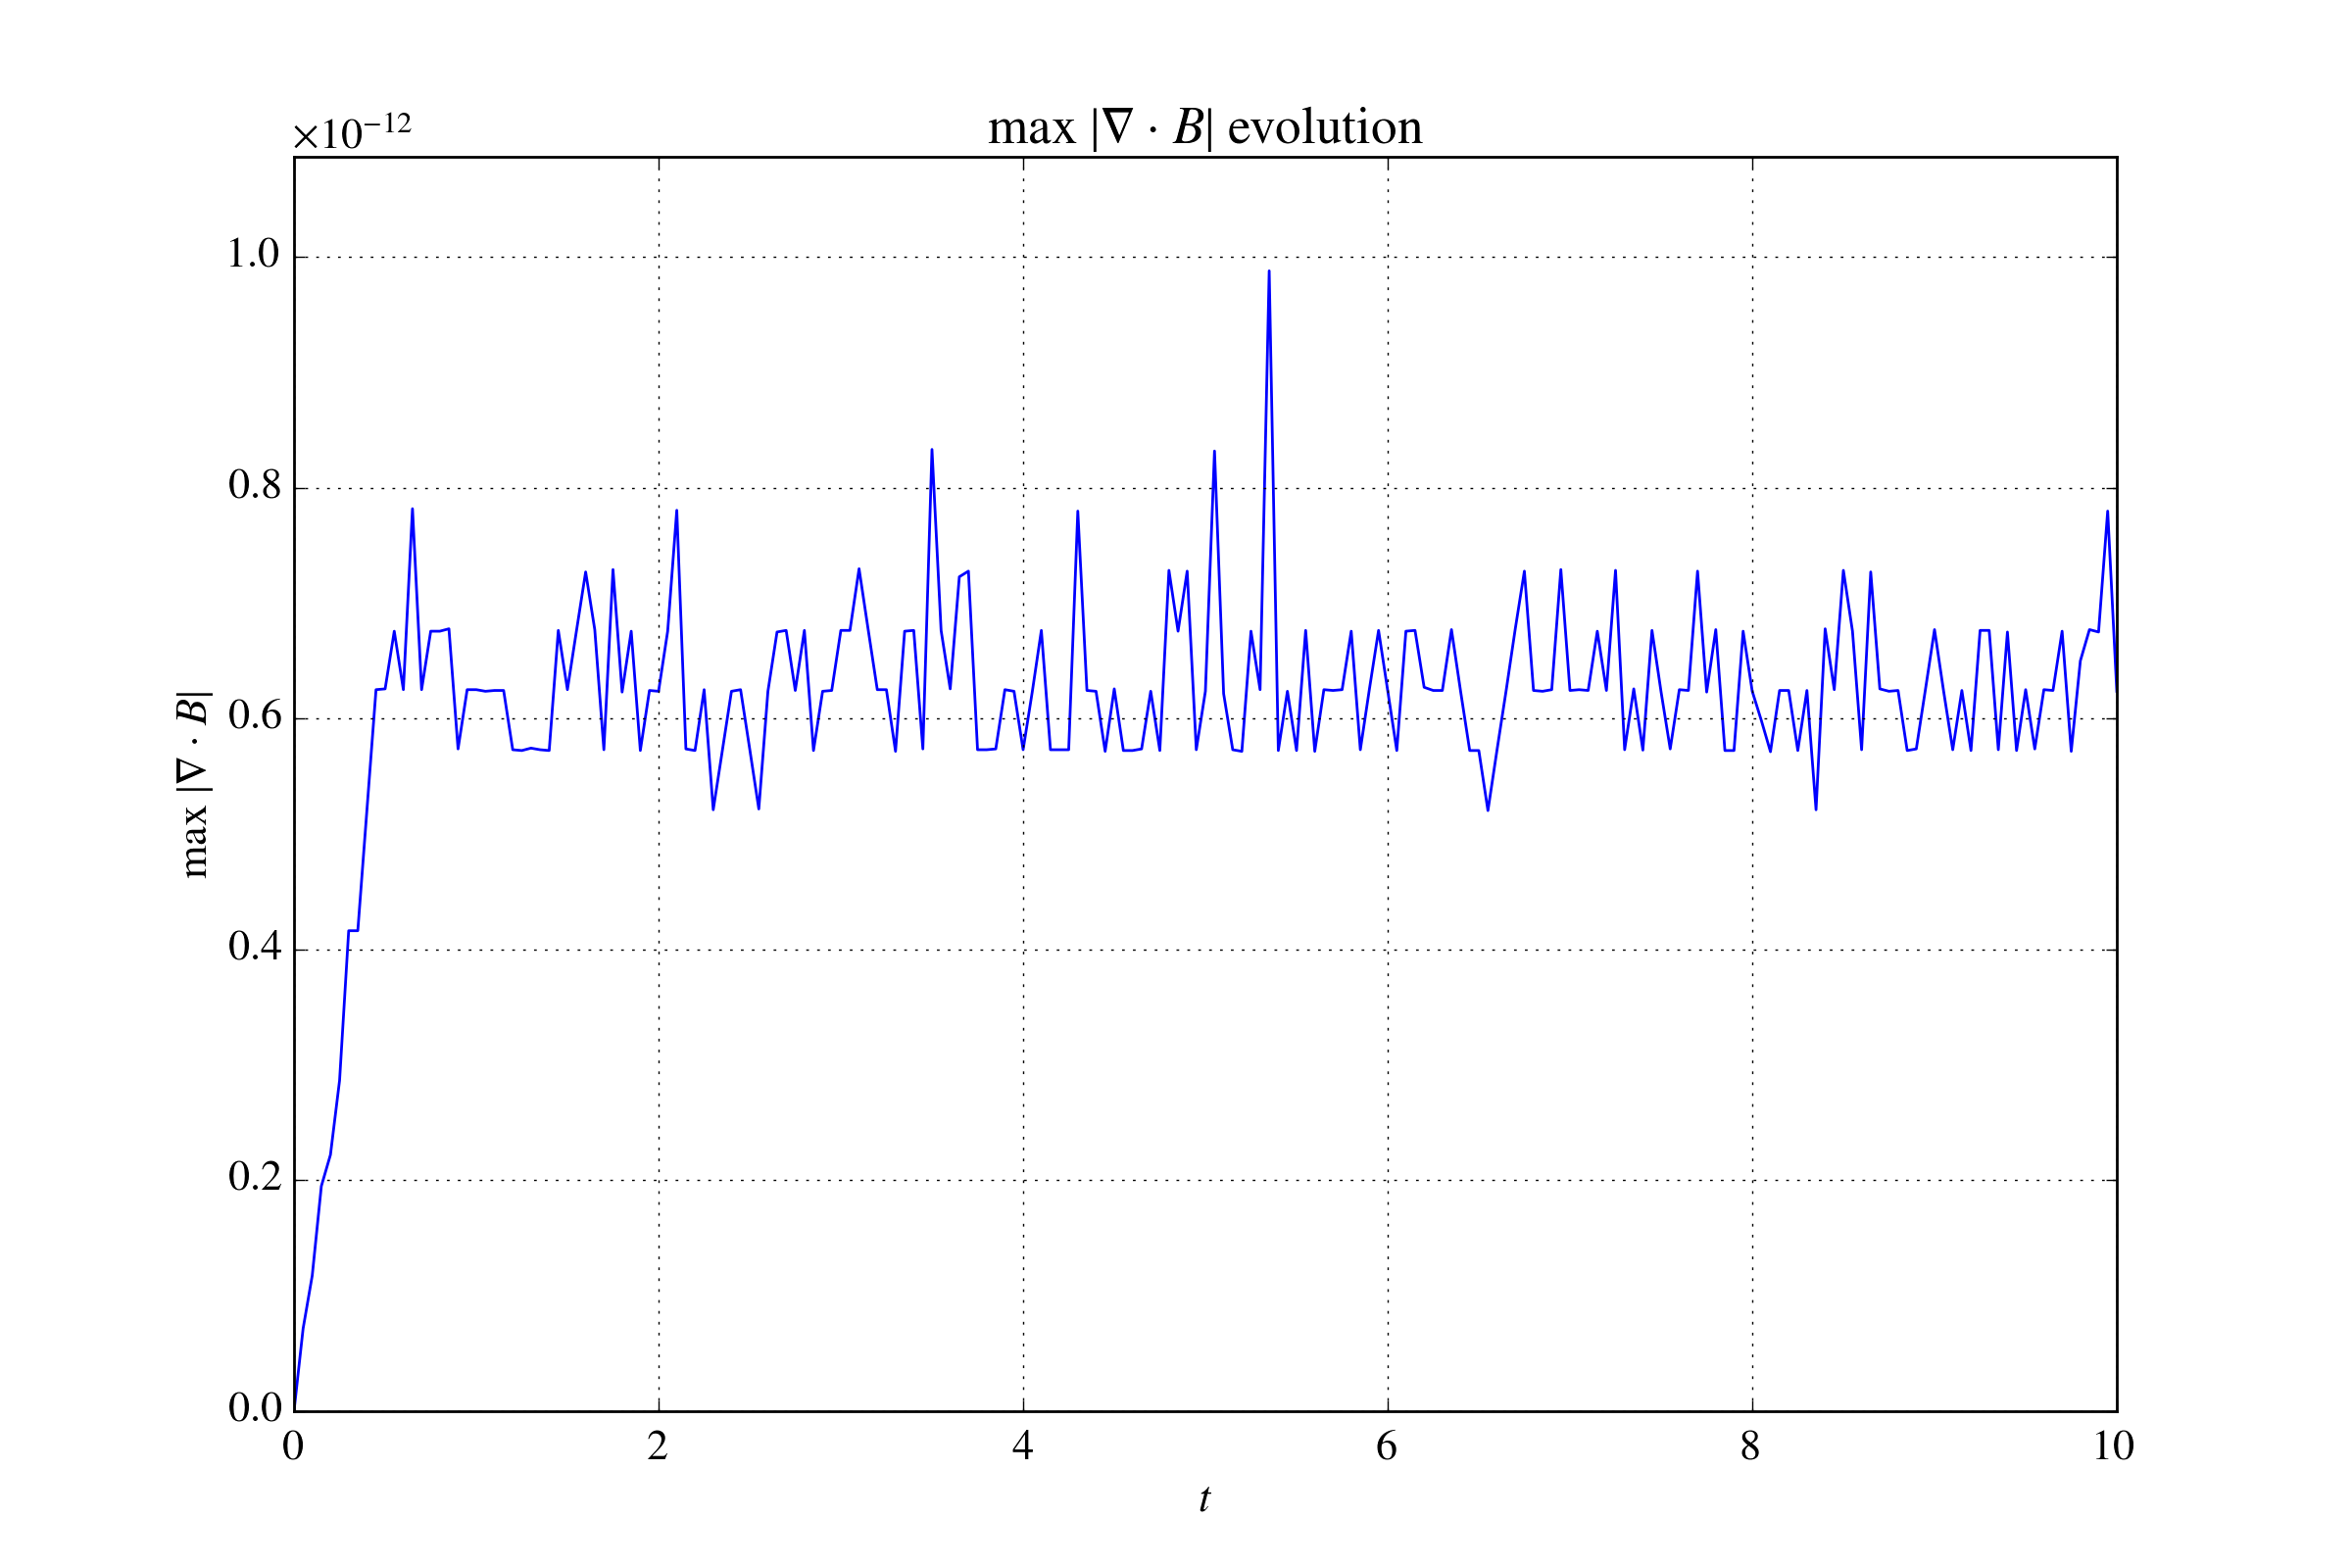
\includegraphics[width=0.8\linewidth]{simulations/divBRe50N100Chi05Cpm5T10fps20.png}
\captionof{figure}{$\nabla\cdot\mathbf{B}$ máximo calculado na malha}
\end{center}

\begin{center}
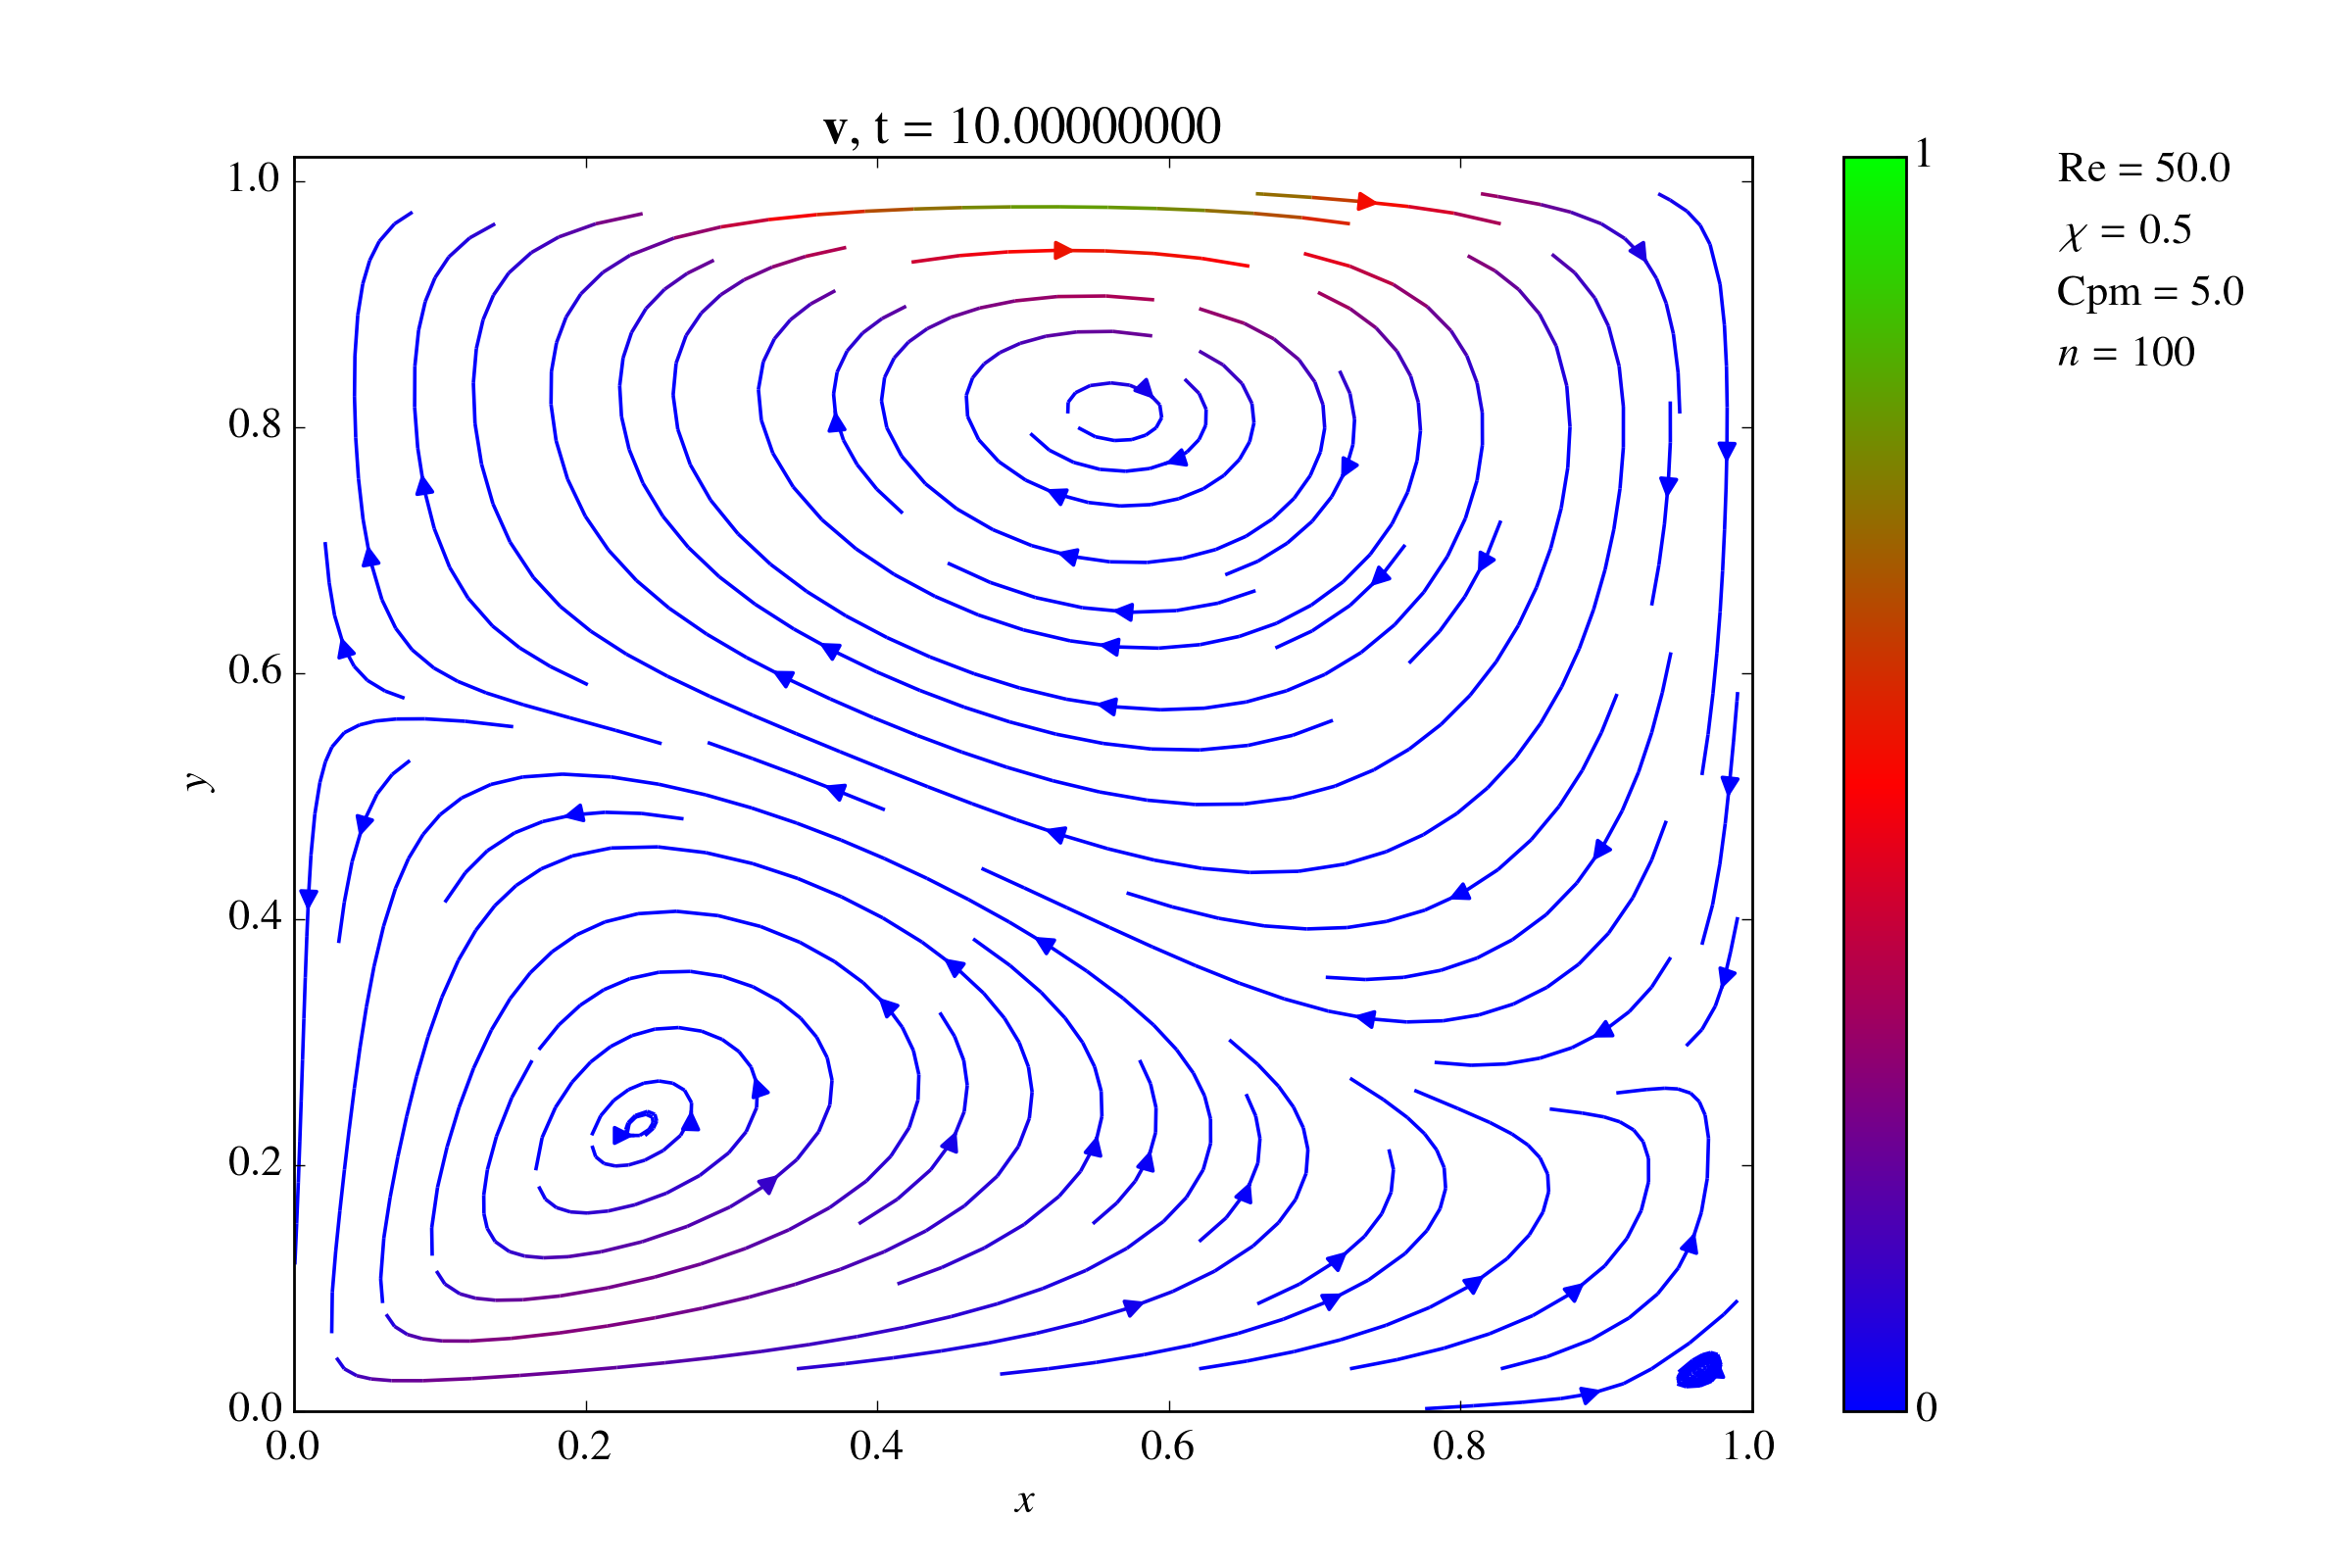
\includegraphics[width=0.8\linewidth]{simulations/vRe50N100Chi05Cpm5T10fps20.png}
\captionof{figure}{Linhas de velocidade em regime com campo aplicado}
\end{center}

\begin{center}
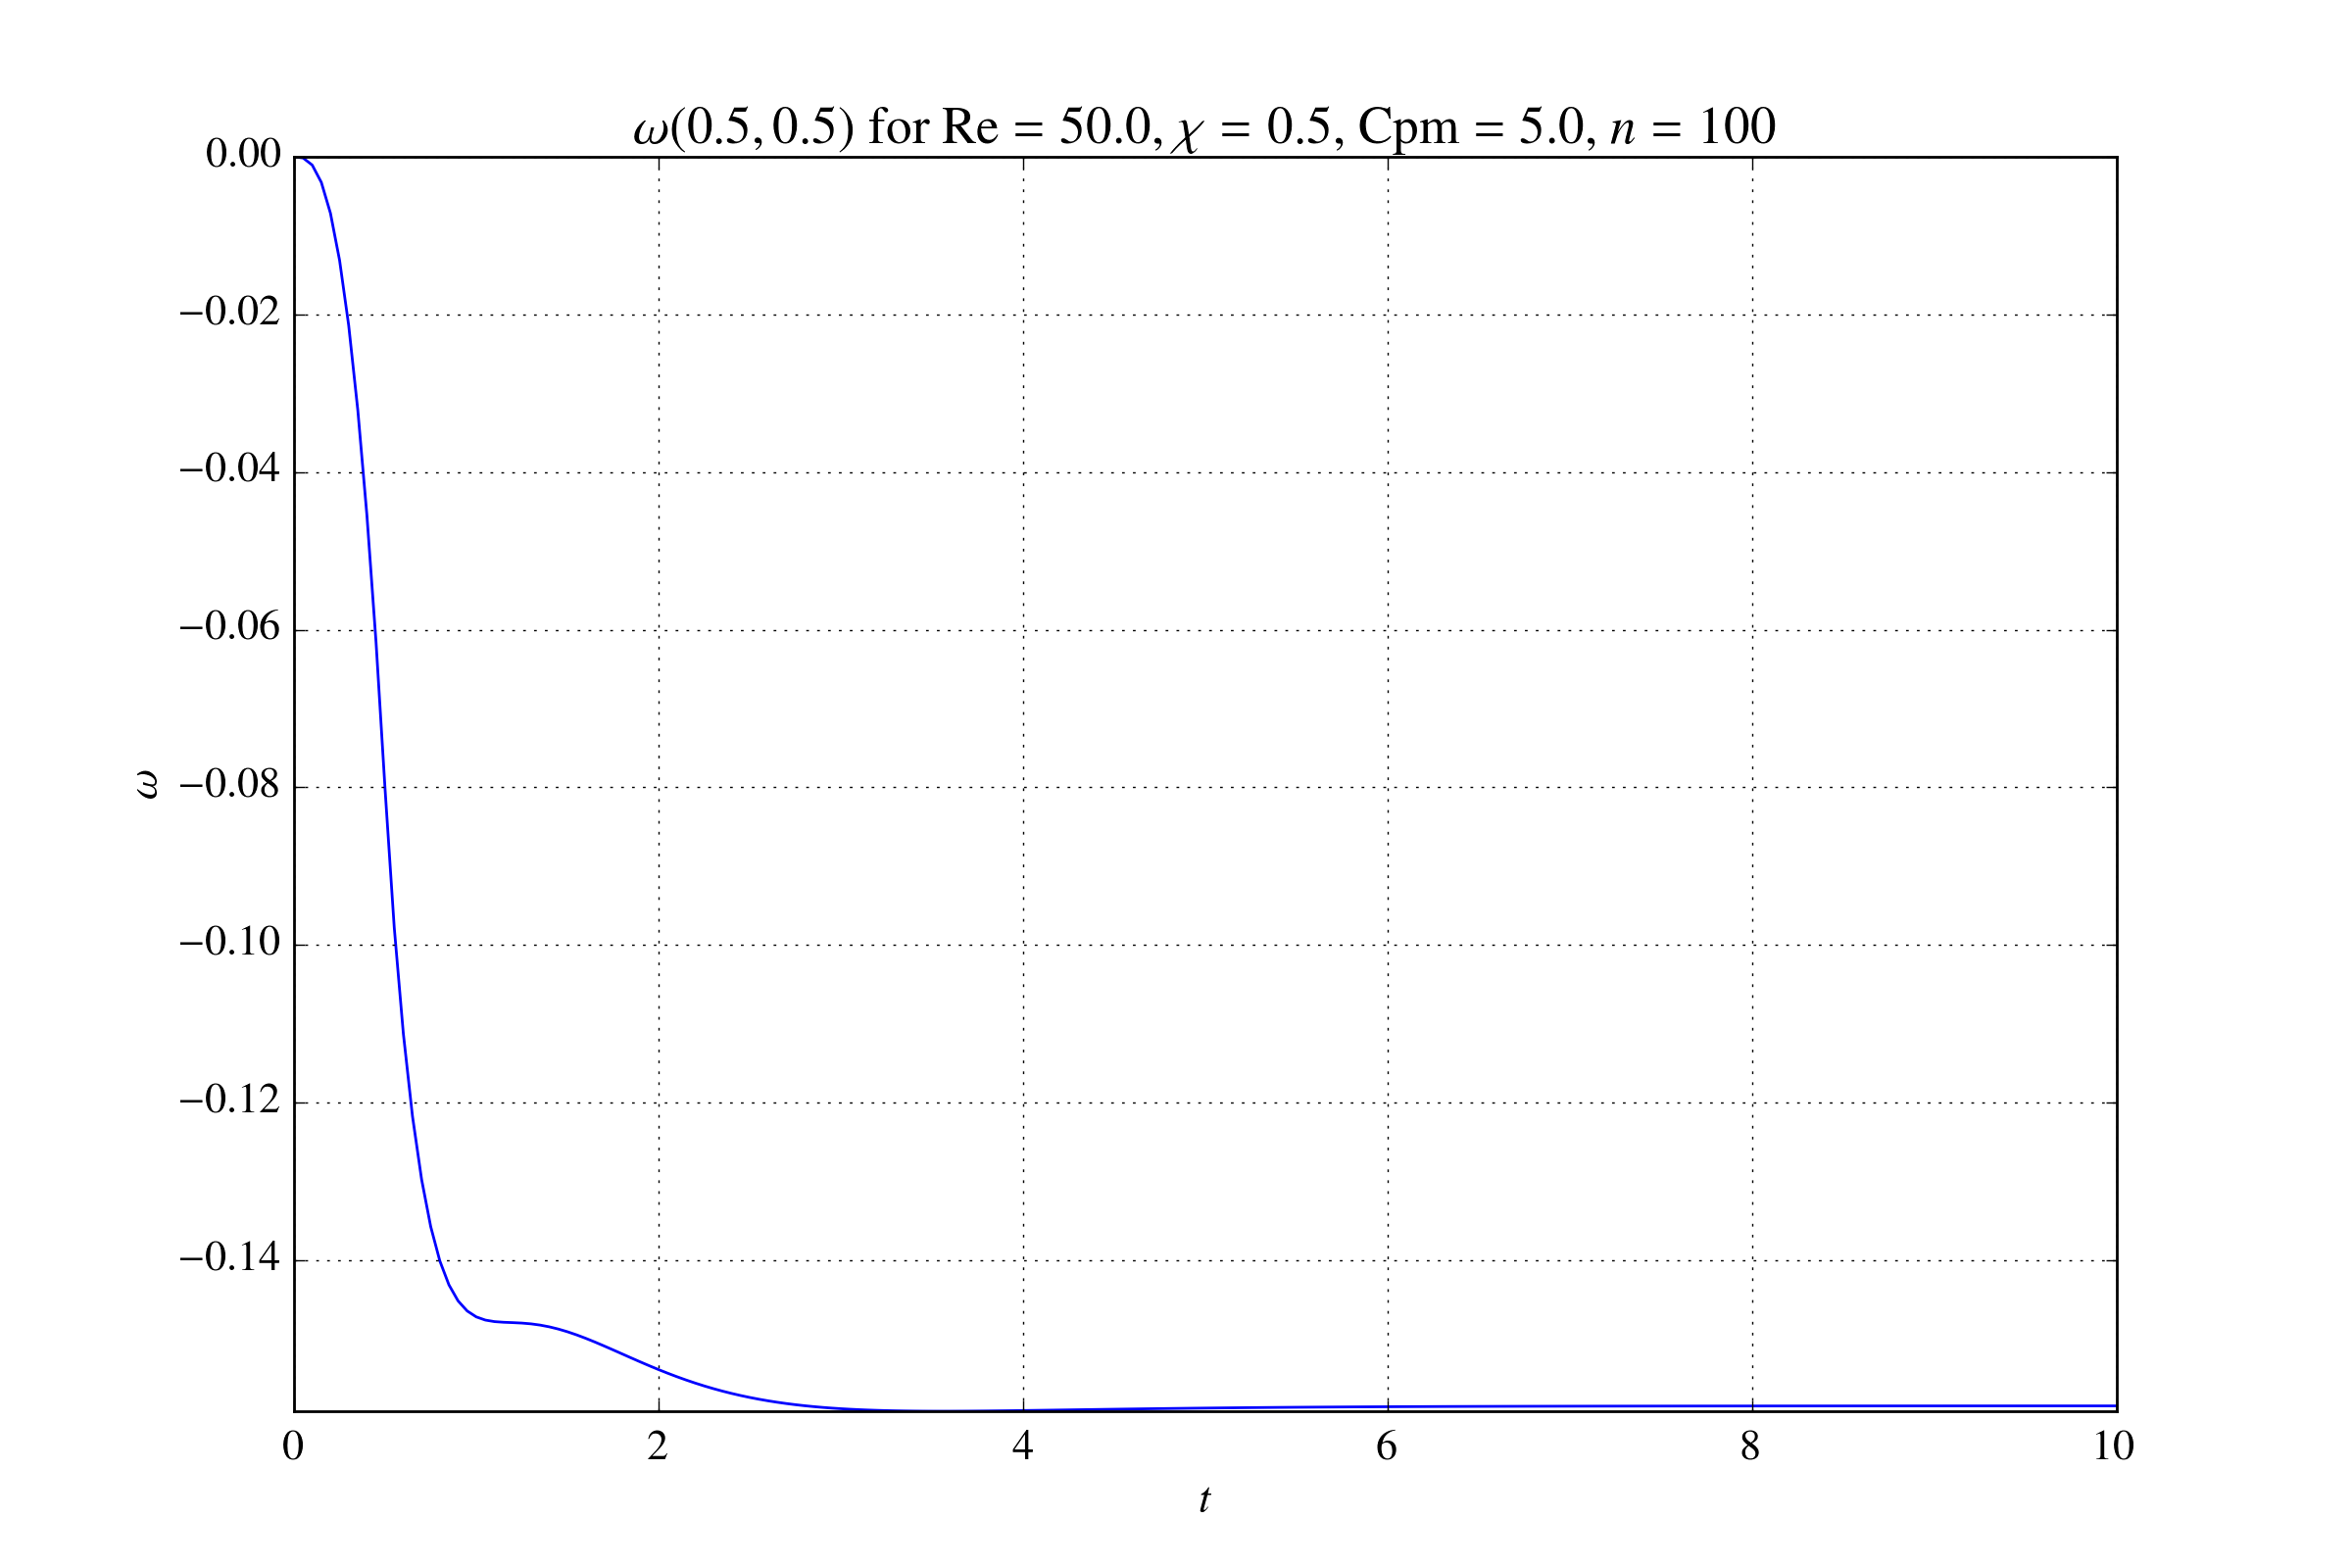
\includegraphics[width=0.8\linewidth]{simulations/vortRe50N100Chi05Cpm5T10fps20.png}
\captionof{figure}{Evolução da vorticidade em (0.5,0.5) com campo aplicado}
\end{center}

\begin{center}
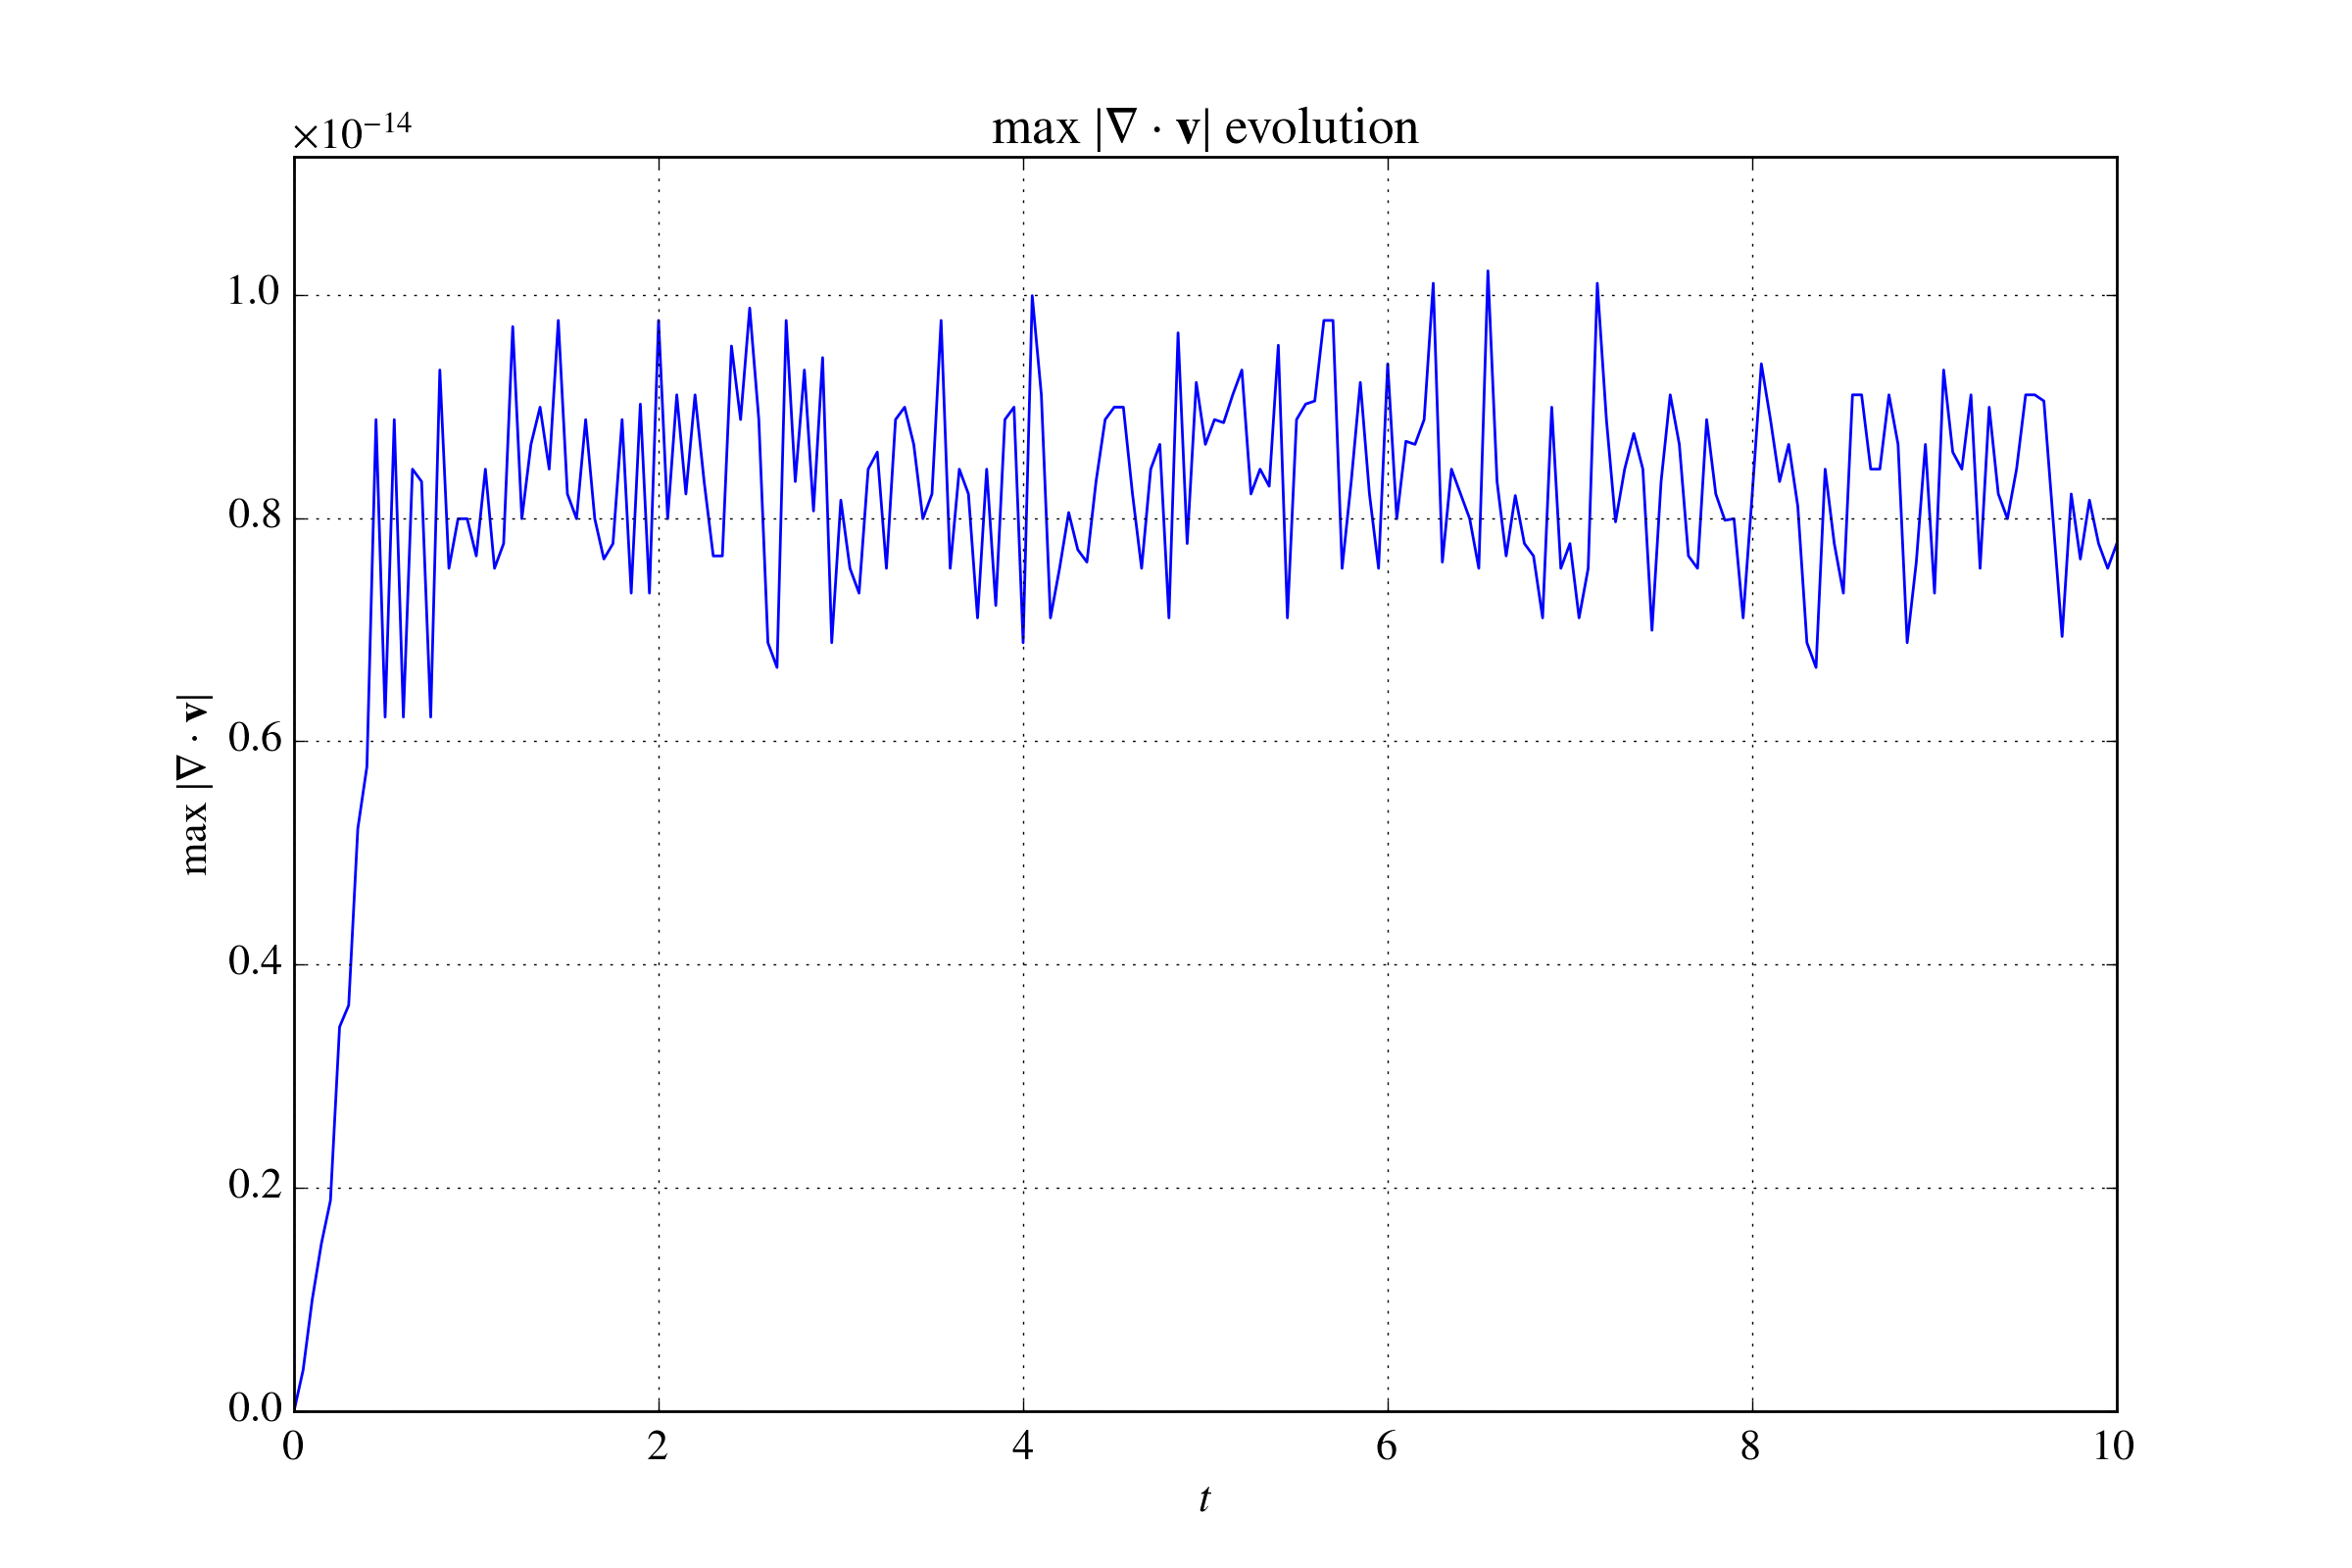
\includegraphics[width=0.8\linewidth]{simulations/divVRe50N100Chi05Cpm5T10fps20.png}
\captionof{figure}{$\nabla\cdot\mathbf{v}$ máximo calculado na malha}
\end{center}

\end{multicols}
}

%----------------------------------------------------------------------------------------
%	FUTURE RESEARCH
%----------------------------------------------------------------------------------------

\headerbox{5. Future Research}{name=futureresearch,column=1,span=1,aligned=references,above=bottom}{ % This block is as tall as the references block


\begin{itemize}
  \item Integrate NiosII-cache with fingerprinting unit and a uTLB (micro-TLB)
  \item Assess whether overall system satisfies time-constraints
  \item Identify possible sources of misbehaving 
  \item Assess perfomance compared to using a scratchpad instead of a cache
\end{itemize}

\vspace{0.1em}
}



%%----------------------------------------------------------------------------------------
%%	CONCLUSION
%%----------------------------------------------------------------------------------------
%
%\headerbox{6. Conclusion}{name=conclusion,column=2,below=anotherresult,bottomaligned=method}{ % This block's bottom aligns with the bottom of the other2 block
%
%\begin{itemize}
%  \item A cache was successfully designed in SystemVerilog, tested and then integrated with the Nios II processor.
%  \item The placement of this memory in between CPU and Main Memory indeed speeds up the system.
%  \item With the cache done, further research with fingerprinting is allowed and analysis of the interactions between cache, fingerprinting unit and uTLB are made possible.
%
%\end{itemize}

%}

%----------------------------------------------------------------------------------------

\end{poster}

\end{document}
